\section{Scope and Assumptions}
\label{sec:scope}

The goal of Tappan Zee Bridge is to find points at which to interpose
for active introspection. This goal led us to define the notion of a tap
point, the context from which a memory access occurs. In this section,
we explore how our definition of a tap point and our focus on active
introspection shape the scope of our work.

First and most obviously, our focus on memory accesses necessarily
limits our scope to information that is read from or written to RAM at
some point. Although this is quite broad, there are notable exceptions.
For example, TRESOR~\cite{Muller:2011} performs AES encryption without
storing the key or encryption states in RAM by making clever use of the
x86 debug registers and the AES-NI instruction set. Aside from such
special cases, however, this assumption is not particularly limiting.

Second, our choice of dynamic analysis limits us to locating
introspection points for events that can be reliably stimulated within
our system. It also means that the tap points we find may require some
validation to ensure that the event they capture has the same semantics
as the one being sought; this piece is currently done by hand.
In many cases, a few minutes of manual examination of the code
surrounding the tap point is all that is required to verify few sets
ought to be merged for better results. This is quite reasonable
compared with the alternative of a fully manual technique.

Third, our goal of finding tap points suitable for active introspection
motivates a design that treats memory accesses at tap points as sources
of \emph{streaming} data. Our algorithms, therefore, typically work in a
streaming fashion as the system executes, remembering only a fixed
amount of state for each tap point. Although this is a natural fit for
active introspection, where events should be reported as soon as
possible, it makes handling data whose \emph{spatial} order in memory
differs from its \emph{temporal} order as it is accessed more difficult.

Finally, the use of calling context in the definition of a tap point
raises the question of how much context is necessary or useful. Our
current system uses only the most recent caller, but we have seen
both situations where this is not enough and where it is too much.
Overall, however, one level of calling context has proved to be a
reasonable choice for a wide variety of introspection tasks.

\begin{figure}[t]
    \begin{center}
        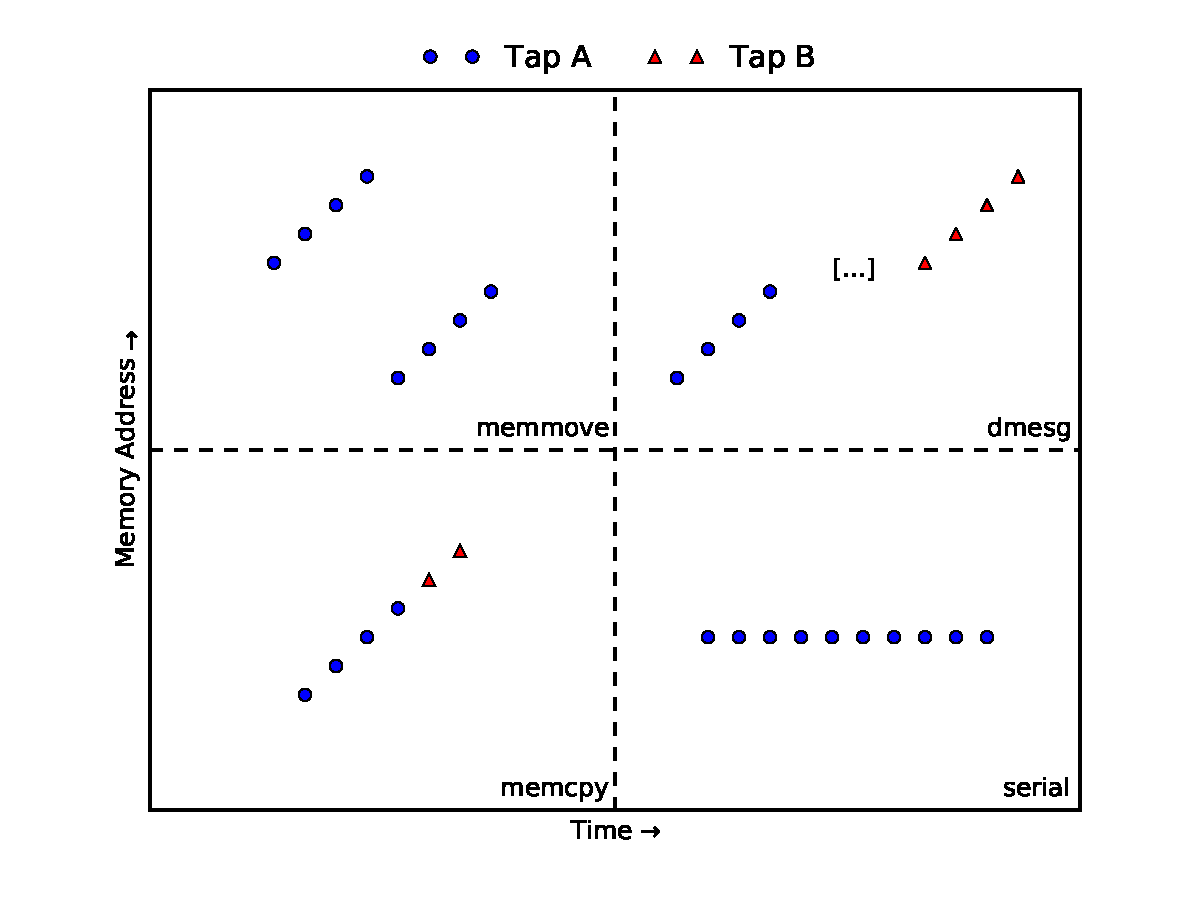
\includegraphics[width=3.2in]{figures/memaccess.pdf}
    \end{center}
    \caption{Patterns of memory access that we might wish to monitor
    using TZB. From left to right and top to bottom: an implementation
    of \texttt{memmove} that copies data backward in 4-byte chunks; two
    tap points that both write to the Linux system log (\texttt{dmesg})
    buffer; an implementation of \texttt{memcpy} that copies data in
    4-byte chunks, copies any remaining bytes one at a time from a
    different tap point; a tap point that writes data one character at
    a time to a serial port. In this diagram, time is represented in
    units of the number of memory accesses.}
    \label{fig:memaccess}
\end{figure}

To better illustrate the boundaries of our technique, consider
Figure~\ref{fig:memaccess}, which plots the address of data written by
different tap points over time for four patterns of memory access. In
the bottom two quadrants, we have cases that are challenging, but
currently well-supported by TZB. In the bottom-left, a standard
\texttt{memcpy} implementation on x86 makes a copy in 4-byte chunks
using \texttt{rep movsd}, and then does a two-byte \texttt{movsw} to get
the remainder of the string. Because the access occurs across two
different instructions, TZB sees two different tap points. Our tap point
correlation mechanism correctly deduces that the accesses are related,
however, because they operate on adjacent ranges in a short span of
time.

The case shown in the bottom right quadrant would be tricky if we looked
only at memory access spatially and not temporally. Here, a utility
function writes data out to a serial port by making one-byte writes to a
memory-mapped I/O address.\footnote{Although not reported in this paper,
this case is one we actually encountered while experimenting with an
embedded firmware.} Because TZB sees these memory writes in
temporal order, ignoring the address, the data is seen normally and the
analyses we describe all operate correctly.

The upper quadrants show cases that are currently not handled by TZB. In
the upper left, \texttt{memmove} copies a buffer in reverse order when
the source and destination overlap. Thus, when viewed in temporal order,
a copy of a string like ``12345678'' would be seen by TZB as
``56781234''. This case is unlikely to be handled by TZB without a
significant redesign, as its view of memory accesses is inherently
streaming.

Finally, the upper right, which represents the case of \texttt{dmesg} on
Linux, is an example of the ``dilemma of context''. Although the
function that writes log data to memory (\texttt{do\_syslog}) is called
from multiple places (creating multiple tap points), it writes to the
same contiguous buffer. Unlike the \texttt{memcpy} case, a significant
amount of time may pass before the next function calls
\texttt{do\_syslog}, and so our tap correlation, which only considers
memory accesses within a fixed time window, will not notice that the tap
points ought to be grouped together. We believe that this case could be
overcome with additional engineering work, but this is left to future
work.
